\begin{figure}[ht]
\centering
%%%%%%%%%%%%%%%% left: the nodal contact sets
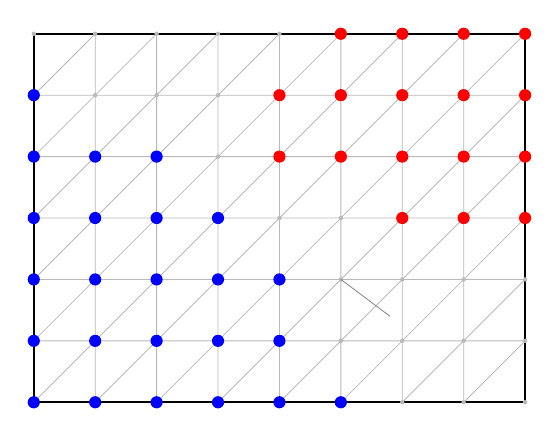
\begin{tikzpicture}[x=0.78cm,y=0.78cm]
  \draw[gray!55,line width=0.3pt]
    \foreach \i in {0,...,8} {(\i,0) -- (\i,6)}
    \foreach \j in {0,...,6} {(0,\j) -- (8,\j)}
    \foreach \i in {0,...,7} {\foreach \j in {0,...,5} {(\i,\j) -- ({\i+1},{\j+1})}};
  \draw[thick] (0,0) rectangle (8,6);
  \foreach \i/\j in {0/6, 1/5, 1/6, 2/5, 2/6, 3/4, 3/5, 3/6, 4/3, 4/6, 5/1, 5/2, 5/3, 6/0, 6/1, 6/2, 7/0, 7/1, 7/2, 8/0, 8/1, 8/2}
    \fill[gray!55] (\i,\j) circle (0.8pt);
  \foreach \i/\j in {0/0, 0/1, 0/2, 0/3, 0/4, 0/5, 1/0, 1/1, 1/2, 1/3, 1/4, 2/0, 2/1, 2/2, 2/3, 2/4, 3/0, 3/1, 3/2, 3/3, 4/0, 4/1, 4/2, 5/0}
    \fill[Blue] (\i,\j) circle (2.2pt);
  \foreach \i/\j in {4/4, 4/5, 5/4, 5/5, 5/6, 6/3, 6/4, 6/5, 6/6, 7/3, 7/4, 7/5, 7/6, 8/3, 8/4, 8/5, 8/6}
    \fill[Red] (\i,\j) circle (2.2pt);
  \node[Blue,fill=white,inner sep=1pt] at (1.6,1.5) {$\Nhbot$};
  \node[Red,fill=white,inner sep=1pt] at (6.5,4.6) {$\Nhtop$};
  \draw[gray,line width=0.3pt] (5,2) -- (5.8,1.4);
  \node[gray,right,inner sep=1pt] at (5.8,1.4) {$\Nh$};
\end{tikzpicture}
\hfill
%%%%%%%%%%%%%%%% right: the element-wise contact sets
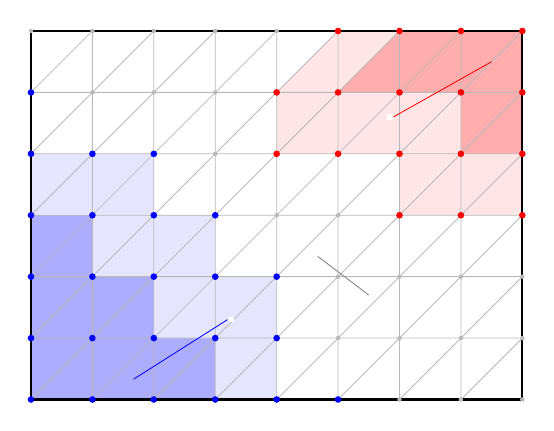
\begin{tikzpicture}[x=0.78cm,y=0.78cm]
  \foreach \i/\j in {0/0, 0/1, 0/2, 1/0, 1/1, 2/0}
    \fill[Blue!32] (\i,\j) -- ({\i+1},\j) -- ({\i+1},{\j+1}) -- cycle;
  \foreach \i/\j in {0/0, 0/1, 0/2, 1/0, 1/1, 2/0}
    \fill[Blue!32] (\i,\j) -- ({\i+1},{\j+1}) -- (\i,{\j+1}) -- cycle;
  \foreach \i/\j in {5/5, 6/5, 7/4, 7/5}
    \fill[Red!32] (\i,\j) -- ({\i+1},\j) -- ({\i+1},{\j+1}) -- cycle;
  \foreach \i/\j in {6/5, 7/4, 7/5}
    \fill[Red!32] (\i,\j) -- ({\i+1},{\j+1}) -- (\i,{\j+1}) -- cycle;
  \foreach \i/\j in {0/3, 1/2, 1/3, 2/1, 2/2, 3/0, 3/1}
    \fill[Blue!10] (\i,\j) -- ({\i+1},\j) -- ({\i+1},{\j+1}) -- cycle;
  \foreach \i/\j in {0/3, 1/2, 1/3, 2/1, 2/2, 3/0, 3/1}
    \fill[Blue!10] (\i,\j) -- ({\i+1},{\j+1}) -- (\i,{\j+1}) -- cycle;
  \foreach \i/\j in {4/4, 4/5, 5/4, 6/3, 6/4, 7/3}
    \fill[Red!10] (\i,\j) -- ({\i+1},\j) -- ({\i+1},{\j+1}) -- cycle;
  \foreach \i/\j in {4/4, 5/4, 5/5, 6/3, 6/4, 7/3}
    \fill[Red!10] (\i,\j) -- ({\i+1},{\j+1}) -- (\i,{\j+1}) -- cycle;
  \draw[gray!55,line width=0.3pt]
    \foreach \i in {0,...,8} {(\i,0) -- (\i,6)}
    \foreach \j in {0,...,6} {(0,\j) -- (8,\j)}
    \foreach \i in {0,...,7} {\foreach \j in {0,...,5} {(\i,\j) -- ({\i+1},{\j+1})}};
  \draw[thick] (0,0) rectangle (8,6);
  \foreach \i/\j in {0/6, 1/5, 1/6, 2/5, 2/6, 3/4, 3/5, 3/6, 4/3, 4/6, 5/1, 5/2, 5/3, 6/0, 6/1, 6/2, 7/0, 7/1, 7/2, 8/0, 8/1, 8/2}
    \fill[gray!55] (\i,\j) circle (0.8pt);
  \foreach \i/\j in {0/0, 0/1, 0/2, 0/3, 0/4, 0/5, 1/0, 1/1, 1/2, 1/3, 1/4, 2/0, 2/1, 2/2, 2/3, 2/4, 3/0, 3/1, 3/2, 3/3, 4/0, 4/1, 4/2, 5/0}
    \fill[Blue] (\i,\j) circle (1.2pt);
  \foreach \i/\j in {4/4, 4/5, 5/4, 5/5, 5/6, 6/3, 6/4, 6/5, 6/6, 7/3, 7/4, 7/5, 7/6, 8/3, 8/4, 8/5, 8/6}
    \fill[Red] (\i,\j) circle (1.2pt);
  \draw[Blue,line width=0.3pt] (1.67,0.33) -- (3.2,1.3);
  \node[Blue,right,fill=white,inner sep=1pt] at (3.2,1.3) {$\Lamhbot$};
  \draw[Red,line width=0.3pt] (7.5,5.5) -- (5.9,4.6);
  \node[Red,left,fill=white,inner sep=1pt] at (5.9,4.6) {$\Lamhtop$};
  \draw[gray,line width=0.3pt] (4.67,2.33) -- (5.5,1.7);
  \node[gray,right,inner sep=1pt] at (5.5,1.7) {$\Thplus$};
\end{tikzpicture}
\caption{Nodal and element-wise contact sets on a demonstration triangulation $\Th$ (incidentally a structured mesh).  Left: the nodal sets $\Nhbot$ and $\Nhtop$ of Proposition~\ref{prop:nodalsign}, with the remaining nodes of $\Nh$ in gray.  Right: the unions $\Lamhbot$ and $\Lamhtop$ of the element sets $\Thbot$ and $\Thtop$ from \eqref{eq:Thsplit}, darker colors, with $\Thplus$ unshaded.  The pale-colored elements have all active vertices, but they do not survive the erosion because their stars $\Uh(T)$ are not fully active.}
\label{fig:nodalelem}
\end{figure}
